% !TeX root = ../../../book.tex

\subsection{像:定义与示例}

回顾函数的定义,我们要求每个输入都有唯一的输出,这确保了函数在其定义域上的每个元素都有定义。那么值域呢?我们仅要求所有输出都属于值域,但未说明值域的``覆盖程度''。函数的像正是为了描述这一特性。如后续示例所示,即使已知值域,精确确定函数的像也并非总是易事。因此,我们才先定义\emph{函数}及其\emph{值域},再引入\emph{像}的概念。所以请不要误解,我们并不是在有意误导你。

\subsubsection*{定义}

\begin{definition}
    设 $A, B$ 为集合,$f:A \to B$ 为函数,且 $X \subseteq A$。

    \dotuline{$X$ 在函数 $f$ 下的像} 记作 $\im_f(X)$,定义为
    \[\im_f(X) = \{b \in B \mid \exists a \in X \centerdot f(a) = b\}\]
    即 $X$ 在函数 $f$ 下的像是 $X$ 中所有``输入''对应``输出''的集合。

    等价定义为
    \[\im_f(X) = \{f(a) \mid a \in X\}\]
    (当函数明确无歧义时,可简写为 $\im(X)$,并将其称为``$X$ 的像''。)

    当我们说 \dotuline{$f$ 的像}时,指的是整个定义域的像,即 $\im_f (A)$。
\end{definition}

此定义适用于定义域的任意子集 $X \subseteq A$,因此可以讨论定义域的任意``部分''或整体的像。后续示例及练习将涉及 $A$ 的真子集 $X \subset A$ 和全集 $A$。

\subsubsection*{一个发现}

请注意,\emph{对任意} $f, A, B$,恒有
\[\im_f(A) \subseteq B\]
此结论\emph{由定义直接得出},因为像通过 $B$ 的元素构造。下一节将探讨 $\im_f(A) = B$ 的情形。

接下来练习识别函数的像。有时需要验证给定像的正确性,有时需要运用特定方法确定函数的像。

\subsubsection*{示例}

\begin{example}\label{ex:example7.3.2}
    定义函数 $g : A \to B$ 为 $A = \{a, b, c, d, e\}, B = \{1, 2, 3, 4, 5, 6\}$ 且
    \[g = \{(a, 2),(b, 3)(c, 3),(d, 1),(e, 6)\}\]
    设 $X_1 = \{a, b, c\}, X_2 = \{a, c, e\}, X_3 = \{c, d, e\}$。

    你可能已经注意到,此函数与上一节示意图定义的函数相同。参考示意图有助于理解下列像集的计算。

    \begin{center}
        {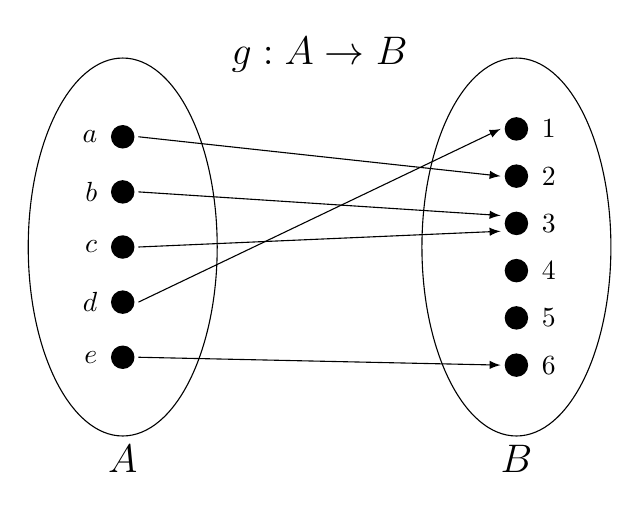
\begin{tikzpicture}[scale=1]
            \foreach \x in  {1,...,6}
            {
                \node at (5, -\x*0.6)[circle,fill,inner sep=3pt]{};
                \draw[shift={(5.2, -\x*0.6)}] node[right] {$\x$};
            }
            \draw (5,-2.1) ellipse (1.2 and 2.4);
    
            \foreach \x/\s in  {1/a,2/b,3/c,4/d,5/e}
            {
                \node at (0, -\x*0.7)[circle,fill,inner sep=3pt]{};
                \draw[shift={(-0.2, -\x*0.7)}] node[left] {$\s$};
            }
            \draw (0,-2.1) ellipse (1.2 and 2.4);
    
            \draw[-latex] (0.2,-0.7) -- (4.8,-1.2); 
            \draw[-latex] (0.2,-1.4) -- (4.8,-1.7); 
            \draw[-latex] (0.2,-2.1) -- (4.8,-1.9); 
            \draw[-latex] (0.2,-2.8) -- (4.8,-0.6); 
            \draw[-latex] (0.2,-3.5) -- (4.8,-3.6);
            
            \node[below] at (0, -4.5){\Large $A$};
            \node[below] at (5, -4.5){\Large $B$};
            \node[above] at (2.5, 0){\Large $g:A \to B$};
        \end{tikzpicture}}
    \end{center}

    \begin{enumerate}[label=(\arabic*)]
        \item $\im_g(\{a\}) = \{2\}$ \\
            请注意此处\emph{大括号}的使用。像永远是\emph{集合}的像,因此写成 $\textcolor{red}{\im_g(a)}$ 是\emph{错误的}。
        \item $\im_g(\{b, c\}) = \{3\}$ \\
            因为 $g(b) = g(c) = 3$。
        \item $\im_g(X_1) = \{2, 3\}$ \\
            因为 $g(b) = g(c) = 3, g(a) = 2$。
        \item $\im_g(X_2) = \{2, 3, 6\}$ \\
            因为 $g(a) = 2, g(c) = 3, g(e) = 6$。
        \item $\im_g(X_3) = \{1, 3, 6\}$ \\
            因为 $g(c) = 3, g(d) = 1, g(e) = 6$。
        \item $\im_g(A) = \{1, 2, 3, 6\}$ \\
            观察示意图中的集合 $B$,可以发现这些值是唯一被函数``命中''的。注意,虽然 $4,5 \in B$,但 $4,5 \notin \im_g(A)$,因此 $\im_g(A) \subset B$,即 $\im_g(A)$ 是 $B$ 的\emph{真}子集)。
    \end{enumerate}
\end{example}

\begin{example}
    考虑液态水的温度范围(以摄氏度为单位)。具体来说,定义集合
    \[C = \{x \in \mathbb{R} \mid 0 < x < 100\}\]
    以及函数 $F : C \to \mathbb{R}$
    \[\forall c \in C \centerdot F(c) = \frac{9}{5}c + 32\]
    $\im_F (C)$ 是什么?其物理意义是什么?

    要解决此问题,我们需要
    \begin{enumerate}[label=(\alph*)]
        \item 通过定义集合来\emph{声明} $\im_F (C)$ 的含义;
        \item 证明该集合\emph{等于} $\im_F (C)$;即二者在集合意义上相等。 
    \end{enumerate}
    
    为此,我们将采用\emph{双向包含论证法}!

    \textbf{解}:定义 $S = \{y \in \mathbb{R} \mid 32 < y < 212\}$。(注意,这表示液态水的温度范围,以华氏度为单位。)我们声称 $S = \im_F(C)$。

    \begin{center}
        \begin{tikzpicture}
            \begin{axis}[
                ymin=0,
                ymax=220,
                xmin=0, 
                xmax=105,
                minor tick num=5,
                axis lines*=middle,
                xtick align=inside,
                ytick align=inside
                ]       
                \addplot[blue, line width=1pt, domain=0:100, samples=2] {x*1.8+32};
            \end{axis}
        \end{tikzpicture}
    \end{center}

    一般来说,很难给出如何提出这种主张的建议。这需要对函数进行一些尝试,可能还需要对其性质有深入洞察。在此例中,我们注意到函数是递增的,即若两个输入值 $c_1 < c_2$,则 $F(c_1) < F(c_2)$。这一结论可从函数图像(见上图)得出,或通过识别其为线性多项式得到。因此,为了确定值域只需计算最小输入值和最大输入值的输出:
    \[F(0) = 0 + 32 = 32 \qquad F(100) = \frac{900}{5} + 32 = 212\]
    由此定义集合 $S$(注意:由于 $0 \notin C$ 不在定义域内,不等式中必须使用``$<$'')。我们特意命名该集合以便后续引用,避免隐含假设其为函数的像——这是微妙而重要的区别!现在,我们来证明该主张。

    \begin{proof}
        首先,证明 $I\im_F (C) \subseteq S$。(即证明函数 $F$ 的每一个输出实际上都满足 $S$ 定义中的不等式。)

        (为此,我们将从 $\im_F (C)$ 的任意元素出发,利用像的\emph{定义}来引入\emph{定义域}中的元素。)

        设 $y \in \im_F (C)$ 为任意固定元素。根据像的定义,这意味着 $\exists x \in C$ 满足 $F(x) = y$。给定这样的 $x$。

        由 $C$ 的定义可知 $ 0 < x < 100$。由 $F$ 的定义可知 $F(x) = \frac{9}{5}x + 32$。由于乘以一个\emph{正数}对加法不会改变不等号的方向,因此可以推导出
        \[ \frac{9}{5} \cdot 0 + 32 < F(x) <  \frac{9}{5} \cdot 100 + 32\]
        化简后得
        \[32 < F(x) < 212\]
        因此,$F(x) \in S$,即 $y \in S$。故 $\im_F(C) \subseteq S$。\\
        
        接着,证明 $S \subseteq \im_F (C)$。(即证明 $S$ 的每一个元素实际上都通过某种方式由函数 $F$ 得到。这相当于证明一个存在性命题,即定义域中存在某个元素。)

        设 $s \in S$ 为任意固定元素。由 $S$ 的定义可知 $S \in \mathbb{R}$ 且 $32 < s < 212$。我们需要证明 $\exists c \in C \centerdot F(c) = s$。

        (通过一些演算可以很容易完成。我们提出了以下思路:只需用 $s$ 表达 $c$ 并求解 $c$……)

        定义 $c = \frac{5}{9}(s-32)$。

        我们要证明 $c \in C$。利用 $s$ 的已知信息并带入不等式,可得
        \begin{align*}
            32 < s < 212 &\implies 0 < s - 32 < 180 \\
            &\implies 0 < \frac{5}{9}(s - 32) < \frac{5}{9} \cdot 180 = 100 \\
            &\implies 0 < c < 100
        \end{align*}

        因为 $c \in \mathbb{R}$,因此 $c \in C$。

        接下来我们证明 $F(c) = s$。不难发现
        \begin{align*}
            F(c) &= \frac{9}{5}c + 32 = \frac{9}{5}\Big(\frac{5}{9}(s-32)\Big)+32\\
            &= (s - 32) + 32 = s
        \end{align*}

        这证明了 $s \in \im_F (C)$,因此 $S \subseteq \im_F (C)$。\\

        综上,利用双向包含论证,我们得到结论 $S = \im_F (C)$。
    \end{proof}
\end{example}

上面证明的后半部分确实较为复杂,这在类似证明中很常见。在选择候选值 $c$ 时,我们本质上需要``逆转''函数 $F$ 的过程,即根据给定输出 $s$ 寻找输入 $c$。当函数涉及实数的数值运算时,最佳方法是建立目标等式,例如
\[\frac{9}{5}c + 32 = s\]
并通过求解得到 $c$。由于该函数是线性的,此过程仅产生唯一的 $c$ 值;但在一般情况下,可能会得到多个符合条件的候选值。完成证明仅需一个有效值,因此任选其一即可。不过,寻找候选值的难度取决于具体问题:有时函数并非定义在数集上,此时需要借助更抽象的思路构造候选元素。总之,一切都取决于具体情况,多加练习便能驾轻就熟!

回到这个像代表什么这个问题,由于定义域表示液态水的摄氏温度,因此像实际上对应液态水的华氏温度。

再考察一个证明函数的像属于特定集合的例子。\\

\begin{example}
    定义 $f : \mathbb{R} \to \mathbb{R}$ 为
    \[\forall x \in \mathbb{R} \centerdot f(x) = \frac{x^2}{1+x^2}\]
    让我们来确定函数的像 $\im_f (\mathbb{R})$,并证明结论!

    在这里,我们需要再次借助一些外部策略和直觉来识别函数的像。我们可以使用微积分或代数方法来绘制该函数的图像,然后试着猜测出函数的像。如果你愿意,可以试试。最终你会得到如下函数图像:

    \begin{center}
        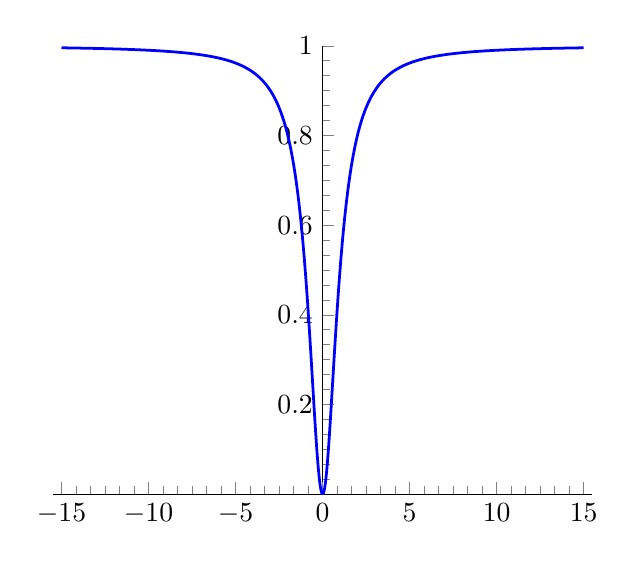
\begin{tikzpicture}
            \begin{axis}[
                ymin=0,
                ymax=1,
                xmin=-15.5, 
                xmax=15.5,
                minor tick num=5,
                axis lines*=middle,
                xtick align=inside,
                ytick align=inside,
                extra x ticks={0}
                ]       
                \addplot[blue, line width=1pt, domain=-15:15, samples=300, smooth] {x^2/(1+x^2)};
            \end{axis}
        \end{tikzpicture}
    \end{center}

    不难发现,表达式中分母大于分子。因此,当 $x$ 越来越大时,分子分母相对来说会越来越接近(也就是说,它们的比率接近 $1$)。另外,由于这两项都涉及平方,因此它们都非负,其比率至少为 $0$。综上所述,我们可以得出以下结论:
    \begin{itemize}
        \item 分母恒大于分子,故当 $|x|$ 增大时,函数值趋近于 $1$
        \item 分子分母均非负,故函数值非负
    \end{itemize}
    据此定义集合
    \[T = \{y \in \mathbb{R} \mid 0 \le y < 1\}\]
    并断言 $T = \im_f(\mathbb{R})$。

    沿用前例证明策略。根据前例的经验,证明所声明集合是像的子集(即 $T \subseteq \im_f (\mathbb{R})$)是难点所在。为此需要处理任意元素 $y \in T$,并寻找 $x \in \mathbb{R}$ 使得 $f(x) = y$。建立如下方程并求解 $x$:
    \begin{align*}
        y = \frac{x^2}{1+x^2} &\iff  (1 + x^2)y = x^2 \\
        &\iff y + yx^2 - x^2 = 0 \\
        &\iff (y - 1)x^2 = -y \\
        &\iff x^2=\frac{y}{1-y} 
    \end{align*}
    求解时需要考虑几个关键问题,$\frac{y}{1-y} \in \mathbb{R}$ 吗?是否确定其非负从而保证 $x$ 存在?如何处理可能出现的双根情况?建议先尝试独立完成证明,再参阅下文给出的证明。

    \begin{proof}
        首先,证明 $\im_f (\mathbb{R}) \subseteq T$。

        设 $y \in \im_f (\mathbb{R})$ 为任意固定元素。根据像的定义,$\exists x \in \mathbb{R}$ 使得 $f(x) = y$。给定这样的 $x$。

        由 $x \in \mathbb{R}$ 可知 $x^2 \ge 0$ 且 $0 < x^2+1$,由此可得 $0 < \frac{1}{x^2+1}$。

        由于所有项均非负,将 $0 < x^2+1$ 和 $0 < \frac{1}{x^2+1}$ 相乘得 $0 < \frac{x^2}{1+x^2}$。

        又由 $0 \le x^2 < x^2 + 1$,可得 $\frac{x^2}{x^2+1}<1$。(备注,为什么指出 $x^2>0$ 很重要?不指出可能会出现什么问题?)

        这证明了 $0 \le \frac{x^2}{1+x^2} < 1$。因为 $y = f(x) = \frac{x^2}{1+x^2}$,这等价于 $0 \le y < 1$。

        故 $y \in T$,因此 $\im_f (\mathbb{R}) \subseteq T$。\\

        接着,证明 $T \subseteq \im_f (\mathbb{R})$。

        设 $y \in T$ 为任意固定元素。这意味着 $y \in \mathbb{R}$ 且 $0 \le y < 1$。

        要证明 $y \in \im_f (\mathbb{R})$,需要得到一个 $x$ 满足 $f(x) = y$。

        我们声称 $x = \sqrt{\frac{y}{1-y}}$ 满足。

        请注意 $0 \le y < 1 \implies -y > -1$,所以 $1-y > 0$。由于 $\frac{y}{1-y} \ge 0$ 且 $x \in \mathbb{R}$,因此可以明确定义为平方根,且 $x$ 属于定义域 $\mathbb{R}$。
        
        注意到 $x^2=\frac{y}{1-y}$,所以
        \[f(x) = \frac{x^2}{1+x^2} = \frac{\frac{y}{1-y}}{1+\frac{y}{1-y}}=\frac{\frac{y}{1-y}}{\frac{(1-y)+y}{1-y}}=\frac{\frac{y}{1-y}}{\frac{1}{1-y}}=\frac{y}{1-y} \cdot \frac{1-y}{1} = \frac{y}{1} = y\]

        这证明了 $y \in \im_f (R)$,因此 $T \subseteq \im_f (R)$。\\

        综上,利用双向包含论证,我们得到结论 $T = \im_f (\mathbb{R})$。
    \end{proof}
\end{example}

请注意我们如何解决先前讨论的证明问题:存在两个可行的 $x$ 值(正平方根与负平方根),但我们仅需一个,这里选择正平方根并完成证明。

(问题:若函数仅定义在非负实数上会怎样?仅定义在负实数上呢?这些限制如何影响我们的选择?)\\

\begin{example}
    考虑函数 $p:\mathbb{N} \times \mathbb{N} \to \mathbb{N}$ 定义为
    \[\forall (a, b) \in \mathbb{N} \times \mathbb{N} \centerdot p(a, b) = ab + a\]
    $\im_p(\mathbb{N})$ 是什么?

    此例可能稍显复杂,因为它涉及集合的笛卡尔积,即函数 $p$ 以自然数对为输入并输出自然数。在这种情况下,一个有效策略是先代入一些具体值观察规律,如下表所示,其中左列为 $a$,顶行为 $b$,表格中的值为 $p(a,b)$。

    \begin{center}
        \begin{tabular}{c|ccccc}
              &  1 &  2 &  3 &  4 &  5 \\
            \hline
            1 &  2 &  3 &  4 &  5 &  6 \\
            2 &  4 &  6 &  8 & 10 & 12 \\
            3 &  6 &  9 & 12 & 15 & 18 \\
            4 &  8 & 12 & 16 & 20 & 24 \\
            5 & 10 & 15 & 20 & 25 & 30 \\
        \end{tabular}
    \end{center}

    看起来函数 $p$ ``取得''除 $1$ 以外的所有自然数。特别地,数组第一行显示除 $1$ 以外所有自然数均出现。下文证明将运用这一洞察。

    \begin{proof}
        设 $V = N - \{1\}$。我们声称 $V = \im_p(\mathbb{N} \times \mathbb{N})$。

        首先,证明 $\im_p(\mathbb{N} \times \mathbb{N}) \subseteq V$。

        设 $n \in \im_p(\mathbb{N} \times \mathbb{N})$ 为任意固定元素。这意味着 $n \in \mathbb{N}$ 且 $\exists (a,b) \in \mathbb{N} \times \mathbb{N}$ 使得 $p(a,b)=n$。给定这样的 $(a,b)$。这意味着 $n=ab+a$。
        
        由 $a,b \ge 1$ 可得 $ab \ge 1$,因此 $n = ab + a \ge 2$。根据 $V$ 的定义,这证明了 $n \in V$。

        因此 $\im_p(\mathbb{N} \times \mathbb{N}) \subseteq V$。

        (在继续阅读之前,试着自己写出证明的后半部分!)\\

        接着,证明 $V \subseteq \im_p(\mathbb{N} \times \mathbb{N})$。

        设 $v \in V$ 为任意固定元素。这意味着 $v \in \mathbb{N}$ 且 $v \ge 2$。定义 $(a, b) = (v - 1, 1)$。

        注意到 $v - 1 \ge 1$,故 $v-1 \in \mathbb{N}$,所以 $(a, b) \in \mathbb{N} \times \mathbb{N}$。

        此外,我们还注意到
        \[p(a, b) = p(v - 1, 1) = (v - 1) \centerdot 1 + 1 = v - 1 + 1 = v\]
        
        故 $p(a, b) = v$,所以 $(a,b) \in \im_p(\mathbb{N} \times \mathbb{N})$。
        
        因此 $V \subseteq \im_p(\mathbb{N} \times \mathbb{N})$。\\

        综上,利用双向包含论证,我们得到结论 $V = \im_p(\mathbb{N} \times \mathbb{N})$。
    \end{proof}
\end{example}